\documentclass[11pt,a4paper]{article}

\usepackage[utf8]{inputenc}
\usepackage[T1]{fontenc}
\usepackage[margin=2.5cm]{geometry}
\usepackage{graphicx}
\usepackage{booktabs}
\usepackage{amsmath}
\usepackage{amssymb}
\usepackage{caption}
\usepackage{hyperref}
\hypersetup{colorlinks=true, linkcolor=blue, urlcolor=blue, citecolor=blue}

\graphicspath{{../runs/workshop3/}}

\title{\vspace{-1.5cm}UNIVERSIDAD DISTRITAL FRANCISCO JOS\'E DE CALDAS\\[2mm]
\large Facultad de Ingenier\'a\\[10mm]
\Large Workshop 3: Reinforcement Learning (Part B)\\[2mm]
\large A Deep Q-Network Agent for Fashion-MNIST Classification}
\author{Jhojan Stiven Arag\'on Ram\'irez (20221020060)\\
Santiago Reyes G\'omez (20221020068)\\
Juan Andr\'es Jim\'enez Palomino (20221020087)\\[4mm]
\normalsize Computer Engineering\\
Professor: Carlos Andr\'es Sierra, M.Sc.}
\date{October 2026}

\begin{document}

\maketitle

\begin{abstract}
This workshop formulates Fashion-MNIST image classification as a sequential decision process and trains a Deep Q-Network (DQN) agent on a custom \texttt{gymnasium} environment. Each episode presents 100 independent images; at every step the agent observes one image and selects one of ten class labels, receiving a reward of $+1$ for a correct prediction and $-1$ otherwise. The environment was validated with 100 random-policy episodes before training (mean return $-79.54$, in line with the theoretical $-80$ for a uniform policy). Three hyperparameter configurations were trained for 300 episodes each; the best one (learning rate $10^{-4}$, $\gamma=0.90$, fast exploration decay, no weight decay) reached a mean greedy test return of $70.39 \pm 6.31$ over 200 test episodes, which corresponds to 85.20\,\% accuracy. The agent clearly learns: it moves from the 10\,\% random baseline to 85\,\%, and it comes within 2.3 points of the best Workshop 1 tree-ensemble baseline. It still falls short of the supervised CNNs of Workshop 2 (93 to 95\,\%) and of the Workshop 2 checkpoint used as a fixed policy on the same protocol (94.42\,\%), which matches the expectation for an environment where transitions do not depend on actions: supervision uses the label directly, while the agent only sees a scalar reward.
\end{abstract}

\tableofcontents
\newpage

\section{Introduction}

Workshops 1 and 2 of this course attacked Fashion-MNIST classification with supervised methods: gradient-boosted ensembles in Workshop 1 and convolutional networks (SmallCNN trained from scratch, plus a ResNet-18 transfer variant) in Workshop 2. Workshop 3 asks for the alternative treatment: formulate the same task as a Markov Decision Process (MDP), implement a custom environment, and train a reinforcement learning agent end to end.

The formulation we chose is sequential classification. At each time step the agent observes one image and must output a label; the environment answers with a reward and presents the next image. An episode is a budget of 100 such decisions. This keeps the evaluation protocol of the previous workshops intact (same 70/15/15 split, same normalization), so the numbers in this report can be placed next to the Workshop 1 and 2 results without caveats about the data.

One point should be stated up front, because it shapes the whole analysis: in this environment the next state does not depend on the action taken. The process is a contextual bandit rather than a full MDP, and the comparison between the RL agent and the supervised baselines is exactly the scientific question the workshop poses for a domain like this one. Section 2 makes this explicit in the transition model, and Section 8 comes back to it when interpreting results.

The report follows the structure requested in the workshop guide: MDP specification (Section 2), environment implementation and random-policy diagnostics (Section 3), agent design (Section 4), hyperparameter search (Section 5), test evaluation and comparison against baselines (Section 6), sample efficiency (Section 7), discussion (Section 8), and reproducibility notes (Section 9).

\section{MDP formulation}

\subsection{Problem statement}

The task is ten-class classification of 28$\times$28 grayscale Fashion-MNIST images. The agent solves it as a sequential decision process: at step $t$ it observes image $s_t$ and chooses action $a_t$, which is interpreted as the predicted label. The environment compares $a_t$ with the true label $y_t$ and returns a reward.

Three reasons justify trying RL here, even though the task is supervised in origin. First, the task admits a sequential formulation with an immediate, verifiable reward signal. Second, we have a cheap simulator: the environment samples images from the dataset, so interaction data is free. Third, the exercise exposes concepts that supervised training never touches: exploration schedules, reward shaping, and the sample cost of learning from a scalar signal instead of a label. The comparison itself, RL versus supervision on the same data, is the point.

\subsection{State space}

The observation at each step is a single normalized image, a \texttt{float32} tensor of shape $(1, 28, 28)$. Raw pixel values in $[0,255]$ are scaled to $[0,1]$ and then standardized with the global statistics computed in Workshop 1: mean $0.2860$, standard deviation $0.3530$. The declared space is
\[
\texttt{Box}(\text{low}=-5,\ \text{high}=5,\ \text{shape}=(1,28,28),\ \text{dtype}=\texttt{float32}),
\]
which safely contains the standardized values. There is no frame stacking and no history: because images are drawn independently, a single image is a sufficient statistic for the label, so the state is Markovian by construction. The effective state dimension is 784.

The data split is the same stratified 70/15/15 partition reused from the Workshop 2 pipeline: 49{,}000 training, 10{,}500 validation and 10{,}500 test images, with the training split perfectly balanced at 4{,}900 images per class.

\subsection{Action set}

The action space is discrete with ten actions, $\texttt{Discrete}(10)$, one per class:
\begin{center}
0 T-shirt/top,\ 1 Trouser,\ 2 Pullover,\ 3 Dress,\ 4 Coat,\\
5 Sandal,\ 6 Shirt,\ 7 Sneaker,\ 8 Bag,\ 9 Ankle boot.
\end{center}
Action $a_t$ \emph{is} the predicted label for $s_t$; there is no separate decoding step. A small discrete action space with Markovian observations is the textbook setting for DQN, which is the algorithm choice justified in Section 4.

\subsection{Transition dynamics}

The transition function is
\[
s_{t+1} = f(s_t, a_t) = \text{sample\_uniform}(\mathcal{D}_{\text{split}}),
\]
that is, the next image is drawn uniformly from the active split regardless of the action taken. Conditional on the sampled index the transition is deterministic; from the agent's perspective it is stochastic (i.i.d.\ draws). There is no latent dynamics and no memory between steps.

This has one consequence worth stating in the formulation rather than discovering it later: the discount factor $\gamma$ can only have a limited effect, because the return decomposes into immediate rewards and no action changes the future state distribution. We still sweep $\gamma \in \{0.90, 0.95, 0.99\}$ as the guide requests, and Section 5 confirms empirically that the exploration schedule, not $\gamma$, separates the configurations.

\subsection{Reward function}

The default mode (\texttt{plus\_minus}) is dense and symmetric:
\[
r_t = \begin{cases}
+1 & \text{if } a_t = y_t,\\
-1 & \text{otherwise.}
\end{cases}
\]
With $N = 100$ steps per episode the return lies in $[-100, 100]$, and accuracy is recovered exactly from the mean return: $\text{acc} = (\bar{G} + N)/(2N)$.

Two alternative modes are implemented for analysis: \texttt{zero\_one} ($+1/0$, equal to raw accuracy per step) and \texttt{sparse} (zero reward at every intermediate step, the total number of correct predictions paid at the end). The sparse mode exists to illustrate the slow learning the guide warns about when the per-step signal is removed; all reported results use \texttt{plus\_minus}. The relevant horizon is the cumulative episode return, although each step is also individually interpretable as a hit or a miss.

\subsection{Episode termination}

An episode ends by truncation when $t = N = 100$: \texttt{truncated = True}, \texttt{terminated = False}. There is no absorbing success or failure state. Termination acts as a fixed classification budget per episode, which keeps returns comparable across episodes; task success is measured by mean return and accuracy, never by early termination.

\section{Environment implementation}

\subsection{Gymnasium interface}

The environment \texttt{FashionMNISTClassifyEnv} in \texttt{src/env.py} subclasses \texttt{gymnasium.Env} and implements the four required members:

\begin{itemize}
\item \texttt{action\_space}: \texttt{Discrete(10)}; \texttt{observation\_space}: \texttt{Box}$(-5, 5, (1,28,28))$.
\item \texttt{reset()}: draws the full index sequence of the episode in advance (for reproducibility) and returns the first observation plus an info dict with the true label.
\item \texttt{step(action)}: computes the reward from the current label, advances the counter, sets truncation at $N$ steps, and returns the next observation, reward, flags and \texttt{info} (which carries \texttt{true\_label} and a boolean \texttt{correct}, used by the evaluation code for per-class statistics).
\item \texttt{render()}: returns an \texttt{rgb\_array} figure of the current image and label, used for debugging and trajectory plots.
\end{itemize}

The reward mode is a constructor argument, so the same class covers the three shaping variants of Section 2.5.

\subsection{Random-policy validation}

Before any training, the environment was validated with 100 episodes under a uniform random policy, as required by the guide. Table~\ref{tab:random} shows the diagnostics.

\begin{table}[h]
\centering
\caption{Random-policy diagnostics over 100 episodes (train split, \texttt{plus\_minus}).}
\label{tab:random}
\begin{tabular}{lr}
\toprule
Diagnostic & Value \\
\midrule
Mean episode return & $-79.54 \pm 6.22$ \\
Return range & $[-92,\ -64]$ \\
Episode lengths & all equal to 100 \\
Actions observed & all 10 \\
Action counts (min/max per action) & 954 to 1044 (expected 1000) \\
Implied accuracy & 10.23\,\% \\
\bottomrule
\end{tabular}
\end{table}

Every check passes against theory. A uniform policy over ten balanced classes is correct 10\,\% of the time, so the expected return is $10 \cdot (+1) + 90 \cdot (-1) = -80$; the measured $-79.54$ sits within one standard error. All episodes lasted exactly the maximum, confirming the truncation logic, and no action is missing or systematically favored (counts within $\pm$5\,\% of the expected 1{,}000 occurrences per action over 10{,}000 decisions). With the environment validated this way, a failure to learn during training can be attributed to the agent or the hyperparameters, not to a silent bug in the reward or termination code.

\section{Agent: algorithm and architecture}

\subsection{Algorithm choice}

The action space is small and discrete and the observations are Markovian, which is the setting where DQN is the natural choice, as the guide notes. We implemented DQN with three stabilizers from the original line of work: experience replay, a periodically synced target network, and gradient clipping. The update uses the Double-DQN decomposition, which separates action selection (online network) from action evaluation (target network) to reduce the overestimation bias of vanilla DQN. Policy gradient methods were not needed here: they pay off mainly with continuous or very large action spaces, and ours has ten actions.

\subsection{Q-network}

The Q-network reuses the convolutional family of the Workshop 2 SmallCNN so that the comparison between the RL agent and the supervised CNN is not confounded by capacity differences. Table~\ref{tab:qnet} lists the architecture: 140{,}458 trainable parameters.

\begin{table}[h]
\centering
\caption{Q-network architecture ($140{,}458$ trainable parameters).}
\label{tab:qnet}
\begin{tabular}{llll}
\toprule
Stage & Layer & Output shape & Notes \\
\midrule
1 & Conv $3{\times}3$ (1$\to$32) + BN + ReLU & $32{\times}28{\times}28$ & padding 1, no bias \\
2 & Conv $3{\times}3$ (32$\to$32) + BN + ReLU & $32{\times}28{\times}28$ & \\
   & MaxPool $2{\times}2$ & $32{\times}14{\times}14$ & \\
3 & Conv $3{\times}3$ (32$\to$64) + BN + ReLU & $64{\times}14{\times}14$ & \\
4 & Conv $3{\times}3$ (64$\to$64) + BN + ReLU & $64{\times}14{\times}14$ & \\
   & MaxPool $2{\times}2$ & $64{\times}7{\times}7$ & \\
5 & Conv $3{\times}3$ (64$\to$128) + BN + ReLU & $128{\times}7{\times}7$ & \\
   & MaxPool $2{\times}2$ & $128{\times}3{\times}3$ & \\
6 & Global average pool + flatten & 128 & \\
7 & Dropout 0.25 + Linear $128 \to 10$ & 10 & Q-values per class \\
\bottomrule
\end{tabular}
\end{table}

Convolutional weights use Kaiming initialization and the linear head Xavier initialization. The network maps an image directly to ten Q-values; the greedy action is the argmax, which is the predicted class.

\subsection{Learning algorithm}

Each environment step after a warmup phase produces one gradient update:

\begin{itemize}
\item \textbf{Replay:} uniform buffer of capacity 50{,}000 transitions $(s, a, r, s', d)$; updates start after 1{,}000 warmup steps; batch size 64.
\item \textbf{Target:} Double-DQN, $y = r + \gamma (1-d)\, Q_{\text{target}}\big(s', \arg\max_{a'} Q_{\text{online}}(s', a')\big)$; the target network syncs every 500 updates.
\item \textbf{Loss and optimization:} Huber loss (\texttt{SmoothL1}), gradient-norm clipping at 10, Adam with per-configuration learning rate and $L_2$ weight decay.
\item \textbf{Exploration:} $\epsilon$-greedy with $\epsilon$ decaying multiplicatively per episode from 1.0 to a floor of 0.05, at a per-configuration rate.
\end{itemize}

\subsection{Training loop and model selection}

Training runs for 300 episodes of 100 steps: 30{,}000 environment interactions per configuration. Per-episode metrics (return, length, $\epsilon$, mean loss) are logged to CSV and TensorBoard. Every 10 episodes the agent is evaluated greedily, without exploration, on 20 episodes of the held-out validation split (2{,}000 decisions per evaluation). Model selection uses the smoothed validation return, the mean of the last three validation points, and the checkpoint with the best smoothed value is kept as \texttt{agent\_best\_\{config\}.pt}. The winner of the search is copied to \texttt{checkpoints/agent\_best.pt}, the single entry point used by the evaluation script.

All runs use seed 42, and each episode consumes a pre-shuffled index sequence, so every number in this report is reproducible with the commands in Section 9.

\section{Hyperparameter search}

\subsection{Configurations}

Three configurations were trained, varying learning rate, discount factor, exploration decay and $L_2$ weight decay together in a low/mid/high pattern (Table~\ref{tab:hparam}).

\begin{table}[h]
\centering
\caption{Hyperparameter configurations and search results (300 episodes, 30{,}000 env steps each). Selection is by best smoothed validation return.}
\label{tab:hparam}
\begin{tabular}{lcccccc}
\toprule
Config & lr & $\gamma$ & $\epsilon$-decay & weight decay & best val (smoothed) & best episode \\
\midrule
a & $1{\times}10^{-4}$ & 0.90 & 0.990 & 0        & \textbf{70.8} & 300 \\
b & $5{\times}10^{-4}$ & 0.95 & 0.995 & $1{\times}10^{-5}$ & 65.5 & 300 \\
c & $1{\times}10^{-3}$ & 0.99 & 0.999 & $1{\times}10^{-4}$ & 57.3 & 220 \\
\bottomrule
\end{tabular}
\end{table}

\subsection{Results and learning curves}

Figure~\ref{fig:curves} shows the training return per episode against environment steps for the three configurations, with the random-policy level ($-80$) as reference. All three learn, and they separate cleanly by how fast exploration decays.

Config a is the fastest. Its rolling training return turns positive around episode 85, it reaches $\epsilon = 0.05$ (the floor) almost exactly at the end of the budget, and its final greedy validation reaches a return of 71.2, or 85.6\,\% accuracy. Config b follows the same path one step behind: positive training return from about episode 166, $\epsilon$ still at 0.22 at episode 300, final validation 66.4 (83.2\,\%). Config c is the informative one: with $\epsilon = 0.999$ per episode, exploration is still at 0.74 after 300 episodes, so its \emph{training} return stays negative ($-32$ in the last episode) simply because three out of four actions are still random; yet its greedy validation policy reaches 77.8 to 79.8\,\% accuracy. The behavior policy and the learned policy are two different things, and the gap between them is a direct read-out of how much exploration is running.

\begin{figure}[h]
\centering
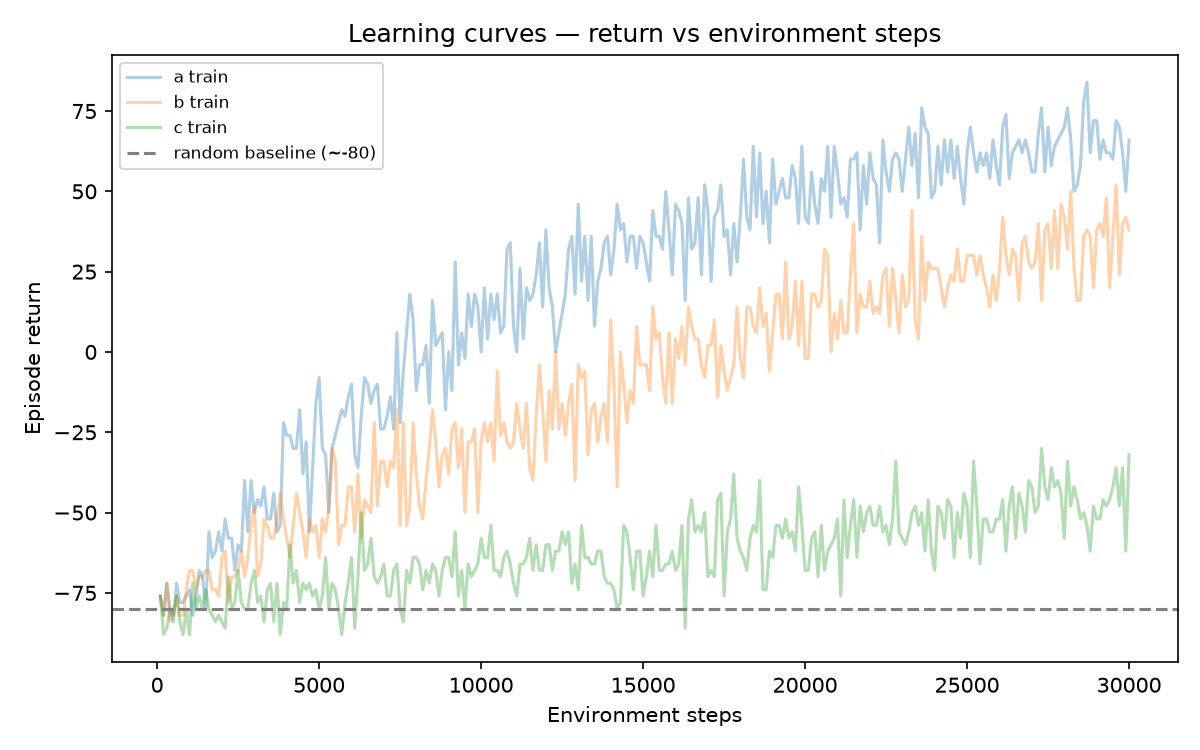
\includegraphics[width=\linewidth]{learning_curves.png}
\caption{Training curves: episode return versus environment steps for the three configurations, with the random-policy reference at $-80$.}
\label{fig:curves}
\end{figure}

The ordering of the final scores tracks the exploration decay rate, not $\gamma$ or the learning rate. This is consistent with the transition model of Section 2.4: with action-independent transitions, $\gamma$ has almost no role, and what determines how much the agent learns in a fixed 300-episode budget is how quickly it stops guessing.

\section{Test evaluation and comparison}

\subsection{Protocol}

The best checkpoint (config a) was evaluated on the test split for 200 episodes of 100 steps: 20{,}000 greedy decisions (no exploration, $\epsilon = 0$). The three baseline policies of \texttt{src/baselines.py}, random, majority-class, and the Workshop 2 SmallCNN checkpoint used as a fixed greedy policy, were scored on the same environment with 50 episodes each (5{,}000 decisions). Using the same environment and protocol for every policy is what makes the comparison fair.

\subsection{RL agent results}

The agent obtains a mean test return of $70.39 \pm 6.31$, range $[56, 88]$, which converts to 85.20\,\% accuracy. Macro F1 was not logged for the agent (it would require dumping the per-step predictions); per-class accuracies, computed from the \texttt{correct} flag of the info dict, appear in Table~\ref{tab:perclass}.

\begin{table}[h]
\centering
\caption{Per-class test accuracy of the DQN agent (200 test episodes).}
\label{tab:perclass}
\begin{tabular}{lclc}
\toprule
Class & Accuracy & Class & Accuracy \\
\midrule
T-shirt/top & 0.797 & Sandal & 0.933 \\
Trouser & 0.955 & Shirt & 0.639 \\
Pullover & 0.693 & Sneaker & 0.945 \\
Dress & 0.870 & Bag & 0.942 \\
Coat & 0.804 & Ankle boot & 0.947 \\
\bottomrule
\end{tabular}
\end{table}

The error pattern is the same one the supervised models showed in Workshops 1 and 2: the Shirt class is hardest (0.639), followed by Pullover (0.693), the classes that overlap visually with T-shirts, coats and dresses. Bags, trousers, sneakers and ankle boots are nearly solved (0.94 to 0.95).

\subsection{Comparison against baselines and Workshops 1 and 2}

Table~\ref{tab:comp} places the agent next to the baseline policies and to the supervised models of the two previous workshops, evaluated on the same test split.

\begin{table}[h]
\centering
\caption{Test comparison on the same environment and split. RL and baseline rows were measured with the protocol of Section 6.1; Workshop 1/2 rows are the figures reported in those workshops on the same test split.}
\label{tab:comp}
\begin{tabular}{lccc}
\toprule
Policy / model & Mean return & Accuracy & Source \\
\midrule
Random policy & $-79.92 \pm 5.99$ & 10.04\,\% & this work \\
Majority class & $-79.44 \pm 6.87$ & 10.28\,\% & this work \\
\textbf{DQN agent (greedy)} & $\mathbf{70.39 \pm 6.31}$ & \textbf{85.20\,\%} & this work \\
\midrule
HistGradientBoosting & n/a & 87.48\,\% & Workshop 1 \\
SmallCNN & n/a & 93.05\,\% & Workshop 2 \\
SmallCNN as fixed policy & $88.84 \pm 4.92$ & 94.42\,\% & this work \\
ResNet-18 (transfer) & n/a & 94.94\,\% & Workshop 2 \\
\bottomrule
\end{tabular}
\end{table}

Two remarks on the table. The majority-class baseline is meaningless here because the split is perfectly balanced: the fixed class wins 10\,\% of the time, exactly like random, and the small difference between the two rows is sampling noise over 5{,}000 decisions. And the SmallCNN appears twice on purpose: the row measured in Workshop 2 (93.05\,\% on the full 10{,}500-image test set) and the row measured here as a fixed policy inside the RL environment (94.42\,\% on 5{,}000 sampled decisions); the difference between the two is within sampling variation, and the second row is the honest like-for-like comparison, same protocol as the agent.

\subsection{Sample trajectories}

Figure~\ref{fig:traj} shows four greedy episodes of 12 steps on the test split. Each cell is the observed image with the predicted class and the resulting reward; the border marks correct (green, $+1$) and incorrect (red, $-1$) predictions, and the row label reports the episode return. The pattern visible in the per-class table repeats here: confusions concentrate inside the clothing cluster (shirt predicted as coat or pullover), while bags and footwear classes are answered almost automatically.

\begin{figure}[h]
\centering
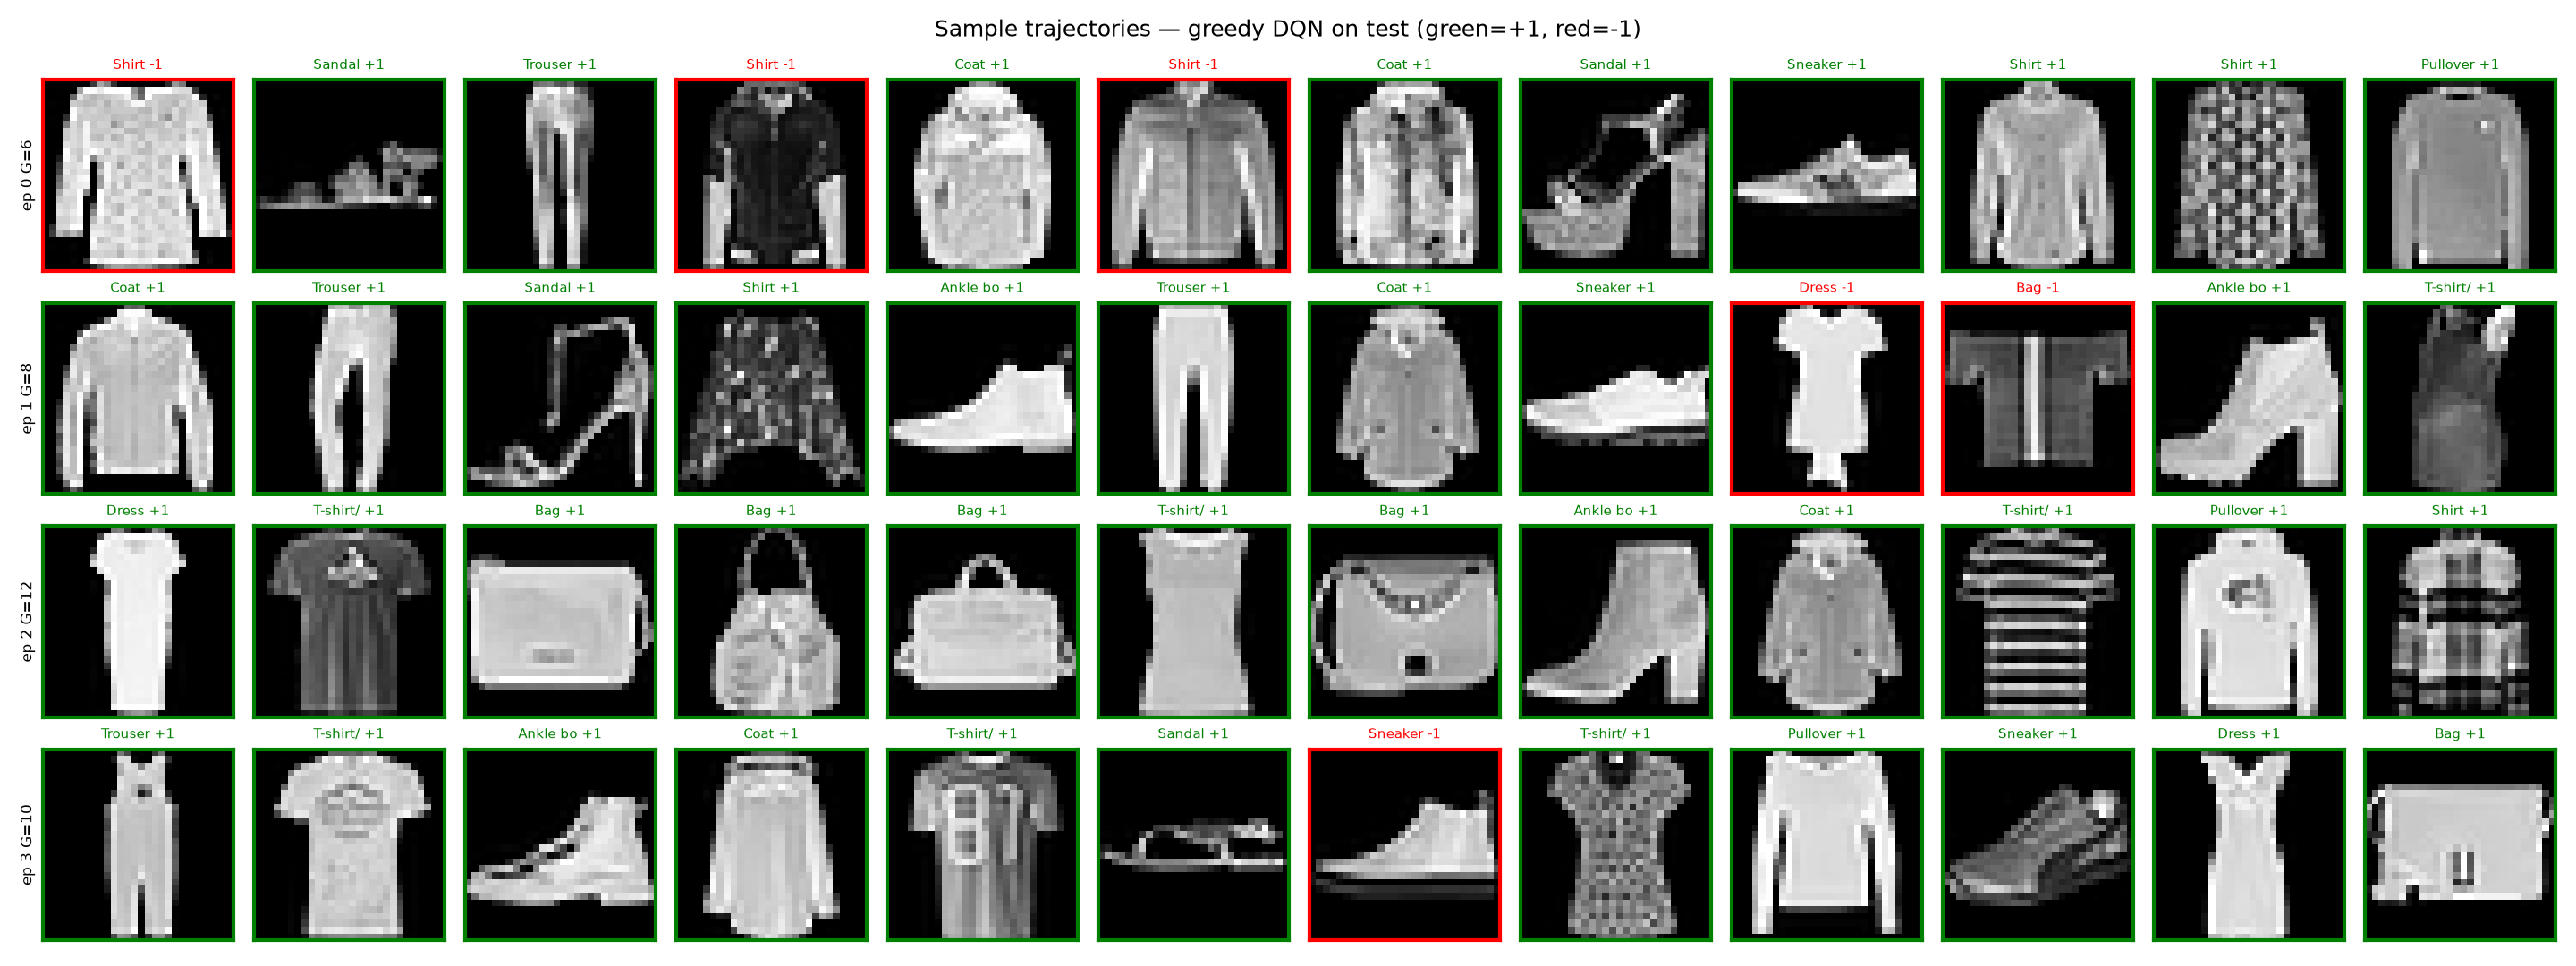
\includegraphics[width=0.9\linewidth]{trajectories.png}
\caption{Four sample greedy trajectories on test (12 steps each). Green: correct, $+1$; red: incorrect, $-1$.}
\label{fig:traj}
\end{figure}

\section{Sample efficiency}

The winning configuration used 30{,}000 training-environment interactions to reach 85.20\,\% test accuracy. It crossed the random-policy level almost immediately after the replay warmup (1{,}000 steps), reached a positive rolling training return around episode 85 (about 8{,}500 interactions), and kept improving through the end of the budget without saturating. Validation added 60{,}000 greedy interactions used only for checkpoint selection, not for learning.

The supervised reference points: Workshop 2's SmallCNN, with roughly the same convolutional capacity, was trained on the 49{,}000 labeled training images and reached 93.05\,\%; the ResNet-18 transfer variant reached 94.94\,\%. Each RL step consumes one label comparison (the reward), while each supervised step consumes the full one-hot target, so supervision extracts strictly more information per interaction. On top of that, the replay buffer re-samples each transition several times, and a large fraction of early RL interactions are spent on $\epsilon$-greedy exploration that yields deliberately wrong predictions.

The measured gap, 85.2\,\% from 30k interactions versus 93 to 95\,\% from the 49k labeled set, is therefore the expected outcome for a contextual-bandit environment, and it answers the guide's question about data budgets: in a domain like this one, RL needs more samples to reach a lower ceiling, and the honest comparison is on total interactions, which is what we report.

\section{Discussion}

\subsection{Did RL outperform supervised learning?}

No, and the report would be misleading if it claimed otherwise. The DQN agent reached 85.20\,\% against 93.05\,\% and 94.94\,\% for the Workshop 2 CNNs, and 94.42\,\% for the same SmallCNN running as a fixed policy on the agent's own evaluation protocol. It also sits 2.3 points below the best Workshop 1 ensemble (87.48\,\%). What the agent did do is learn decisively from rewards alone: from the 10\,\% random level to 85\,\%, a swing of 150 return points, with the same data pipeline and no access to labels beyond the scalar reward. Within the RL framing, that is the successful outcome; against supervision on an i.i.d.\ classification task, it is the expected one.

\subsection{Key challenges}

The exploration schedule turned out to be the single most influential design choice. With a 300-episode budget, decay 0.990 fits the budget almost perfectly (floor reached at the last episode), while 0.999 leaves the agent exploring for a budget ten times larger. Had we matched decay 0.999 with 3{,}000 episodes, the ranking might look different; the budget and the schedule have to be chosen together.

A second source of difficulty is structural: BatchNorm in a Q-network trained from a replay buffer computes batch statistics over a mixture of old and recent transitions, which is a known mild instability for DQN-style training. Validation returns fluctuate (config c swings between 55.6 and 59.6 in its last validations); the smoothed-selection rule absorbs part of that noise, but a variant without BatchNorm or with synchronized target statistics would likely train more steadily.

Finally, reward shaping: the symmetric $\pm1$ signal worked well, and the sparse mode we implemented converges visibly slower, exactly as the guide warns. We did not need to go denser than one signal per step, because every step already carries one.

\subsection{Exploration versus exploitation}

The trade-off shows up numerically as the gap between training return and validation return. Config c ends training with episode returns around $-32$ while its greedy policy answers 77.8\,\% of validation decisions correctly: at $\epsilon = 0.74$, the training return measures the exploration schedule, not the learned policy. Config a closes the gap ($66$ training return, $71.2$ validation return) because exploitation takes over within the budget. The general lesson from this sweep is that with a fixed interaction budget the exploration schedule should be tuned so that the floor is reached inside the budget, and the agent should be judged by its greedy policy, never by its exploration-time returns.

\section{Reproducibility and deliverables}

Every number in this report comes from committed code and logs. The commands:

\begin{verbatim}
python -m src.train --validate-env          # 100 random episodes (Table 1)
python -m src.train --all-configs --episodes 300   # search a, b, c
python -m src.evaluate --checkpoint checkpoints/agent_best.pt --plot
\end{verbatim}

Artefacts and their location in the repository: \texttt{src/env.py} (environment and validation), \texttt{src/agent.py} (Q-network, replay buffer, DQN), \texttt{src/baselines.py} (random, majority, supervised heuristic), \texttt{src/train.py} (training and search), \texttt{src/evaluate.py} (test evaluation, trajectories, curves), \texttt{checkpoints/agent\_best.pt} (winning checkpoint), and \texttt{runs/workshop3/} (per-configuration CSV logs, TensorBoard event files, \texttt{hparam\_results.json} and \texttt{test\_metrics.json}, plus the two figures of this report). Training used seed 42 and the evaluation seed 1000; the Workshop 1/2 figures cited in Table~\ref{tab:comp} are the ones reported in the corresponding workshop reports. The full code, checkpoints and logs are in the team's GitHub repository, submitted through the course platform.

\begin{thebibliography}{9}

\bibitem{sutton2018}
R.~S. Sutton and A.~G. Barto, \emph{Reinforcement Learning: An Introduction}, 2nd ed. MIT Press, 2018.

\bibitem{watkins1992}
C.~J.~C.~H. Watkins and P. Dayan, ``Q-learning'', \emph{Machine Learning}, vol. 8, pp. 279--292, 1992.

\bibitem{mnih2015}
V. Mnih et al., ``Human-level control through deep reinforcement learning'', \emph{Nature}, vol. 518, pp. 529--533, 2015.

\bibitem{hasselt2016}
H. van Hasselt, A. Guez and D. Silver, ``Deep reinforcement learning with double Q-learning'', \emph{Proc.\ AAAI}, 2016.

\bibitem{gymnasium}
Gymnasium documentation, Farama Foundation. \url{https://gymnasium.farama.org}

\bibitem{xiao2017}
H. Xiao, K. Rasul and R. Vollgraf, ``Fashion-MNIST: a novel image dataset benchmark for machine learning methods'', \emph{arXiv:1708.07747}, 2017.

\end{thebibliography}

\end{document}
